\begin{titlepage}
\begin{spacing}{2}

\begin{flushright} %rechtsbündig (Anfang)
	\vspace*{-20mm}
	
\includegraphics[width=\textwidth]{Abbildungen/CoverLogos}
	%
\includegraphics[width=\textwidth]{skizzen/CoverLogos_MZH}
\end{flushright} %rechtsbündig (Anfang)

% der Titel der Arbeit:
\vspace{38mm} {\centering {{\LARGE{Frequenzbasierte Modellierung zur Prädiktion von Personen-Auftrittswahrscheinlichkeiten}}}

\vfill
% hier kommt eine hübsche Grafik hin:
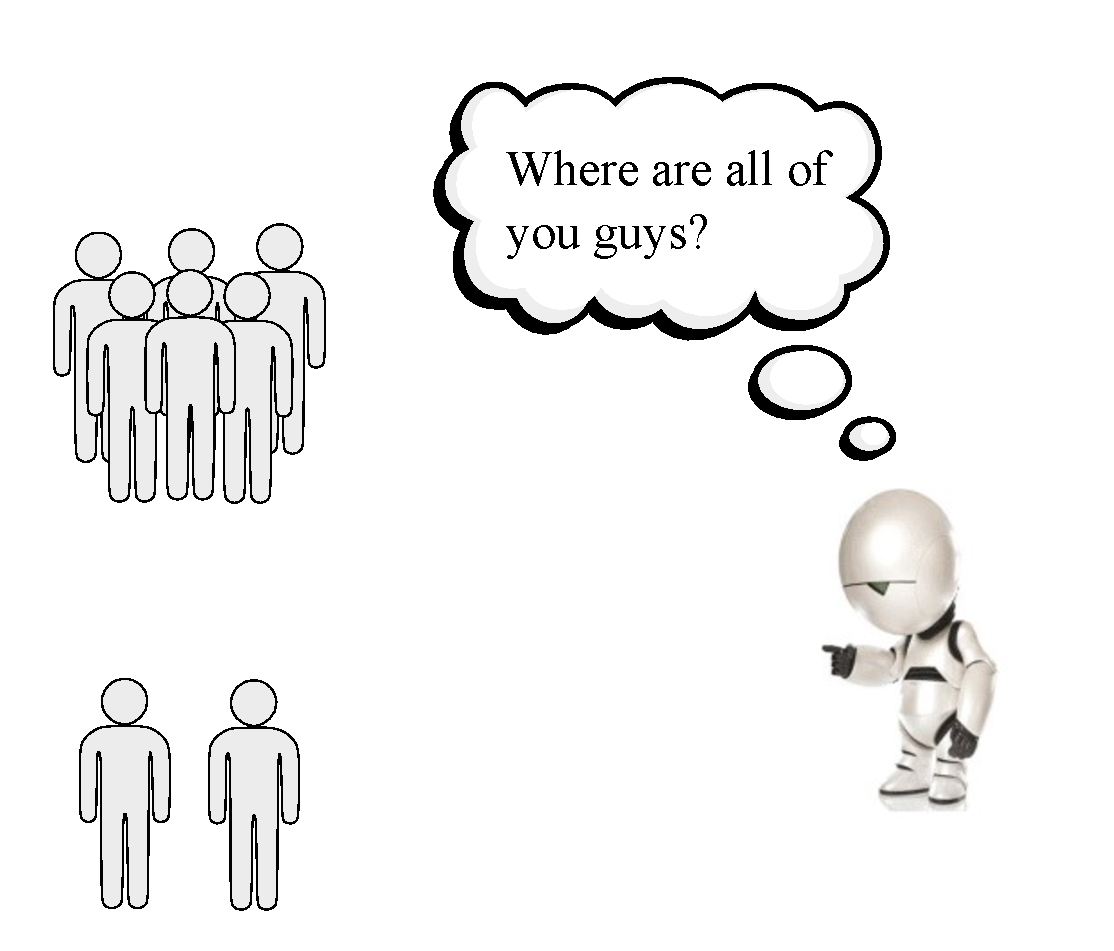
\includegraphics[width = 100mm]{Abbildungen/titelbild_1_0.pdf}


\vfill }
\end{spacing}
\begin{spacing}{1}
\begin{tabular}{l}
 \Large{Studienarbeit S-01/2021-997}
% Die einzutragende Nummer gibt es beim Betreuer!
\end{tabular}

\vspace{5mm}

\begin{tabular}{l}
\large{\Autor}\\
\large{Matrikelnummer \Matrikelnummer}
\end{tabular}

\vspace{5mm}

\begin{tabular}{l}
\large{Hannover, \Datum}
\end{tabular}


\vspace{5mm}
{\large
\begin{tabular}{l l}
Prüfer & Prof. Dr.-Ing. Tobias Ortmaier\\
Betreuer    & Marvin Stüde, M.Sc.\\
\end{tabular}
}

\end{spacing}
\end{titlepage}
\cleardoublepage